%!TeX root=../tese.tex
%("dica" para o editor de texto: este arquivo é parte de um documento maior)
% para saber mais: https://tex.stackexchange.com/q/78101/183146

% Os capítulos de compõem a dissertação/tese, com numeração normal, podem
% ser inseridos diretamente aqui ou "puxados" de outros arquivos.
% Em alguns (raros) casos, pode ser interessante usar \include ao
% invés de \input: https://tex.stackexchange.com/a/32058/183146
%!TeX root=../tese.tex
%("dica" para o editor de texto: este arquivo é parte de um documento maior)
% para saber mais: https://tex.stackexchange.com/q/78101/183146

%% ------------------------------------------------------------------------- %%
\chapter{Introduction}
\label{cap:introduction}

Social networks have all but taken over contemporary daily life. From the
eponymous socializing, to reading news, to expressing ourselves, social media
has creeped into every corner of society. Most of its side-effects, it could be
argued, are positive (shortening distances, political accountability, social
organizing), but they are not perfect institutions.

Social media companies already face significant backlash for their questionable
business model and ethics. Cambridge Analytica's election meddling, Facebook's
subliminal experiments, YouTube's problem with disturbing content marketed at
kids, and Twitter's bot infestation are just a few recent scandals that have put
the societal role of social media into question.

One particular controversy that has taken over public discourse around social
networks is the role that their algorithms might have in radicalizing users,
specially younger ones. The aforementioned experiments conducted by Facebook to
influence people's emotions and the proliferation of more than questionable
videos aimed at children on YouTube are instances that seem to corroborate the
notion that there is something fundamentally wrong with these companies'
algorithms.

News organizations, in general, have been skeptical of social networks.
Journalists and specialists alike argue that social media's algorithms
(specially recommender algorithms) are tuned to peddle conspiracy theories,
extremist views, and false information. This would be the source cause for a
plethora of what they consider contemporary evils: religious extremism,
anti-democratic leaders, widespread depression among teenagers, anti-science
movements, etc.

This narrative, of course, has been questioned for a variety of reasons. Some
say that it is self serving: traditional news organizations are being displaced
by social media and it would be convenient for them to mine the public's trust
in them. Others claim that these recommender algorithms are not to blame for
political polarization and that social networks even have a tendency to favor
more left-wing viewpoints.

The debate around the role of recommender systems in social media radicalization
is still, unfortunately, too recent and based in anecdotes. Since its impacts
are all but universal, more quality research is vital to inform both the public
and opinion makers about if and how much recommendation algorithms influence
social media users.

This dissertation aims to further such research. The rest of Chapter 1 is
dedicated to core concepts covered in the rest of the work, ending in subsection
1.4, which tackles the main hypothesis of this dissertation. Chapter 2 contains
the literature review, Chapter 3 explains the experiments already conducted and
their results, and Chapter 4 is about next steps.

\section{Social Networks}
\label{sec:social_networks}

Social networking services, also referred to as social networks and social
media, are notoriously difficult to define. Some definitions might be too narrow
(excluding instant messaging services), while some might be too broad (including
technologies such as telephone networks). Most definitions include some common
features:

\begin{itemize}
  \item Internet-based
  \item Focus on user-generated content
  \item Users have profiles
  \item Users can connect
\end{itemize}

While social-networking-like applications already existed in Usenet, Geocities,
launched in 1994, is usually regarded as the first major social network.
Friendster and Myspace followed in 2003, with Orkut and Facebook slightly
lagging behind in 2004. Each hit their peak at different moments and different
countries, but Facebook overtook all of them in 2009 when it became the most
popular social networking service in the world, still maintaining the title over
11 years latter at the moment of writing.

Even though all aforementioned social networks are multimedia, that is, users
can post text, photos and videos, some of the most popular services focus on a
specific type of media. For instance, YouTube (2009) centers around videos,
WhatsApp (2009) and WeChat (2011) were originally designed for text-based
communication, and Instagram's (2010) main focus is photos.

Some social media services, very much in agreement with McLuhan's teachings,
have what could be considered a ``style''. Instagram's content, for example,
tends toward more personal (i.e. egoic) photos and videos. As of November 28th,
2020, six of the top 20 most-liked posts on Instagram are from american
socialite Kylie Jenner, consisting of four photos of her daughter and two of her
ex-boyfriend. Even though there are many different niches inside Instagram,
personal posts seam to have an edge over other kinds of content.

Twitter, unlike most other social networks, allows for asymmetrical connections,
meaning users can follow profiles without being followed back. This enables the
emergence of Twitter communities (e.g. Fintwit, Black Twitter) that can be
largely self referential and/or organized around certain subjects. Facebook
users, on the other hand, can belong to groups, user-moderated profiles that
might revolve around any particular topics of interest; there are groups that
organize pet owners and groups that organize neonazis.

Parallel to all other features and idiosyncrasies, there lay the recommendation
algorithms. While a few social networking services (e.g. WhatsApp) do not
recommend any content or profiles to the user, most do and, according to recent
studies, these recommendations have become the main drivers of interactions.

\section{Recommender Systems}
\label{sec:recommender_systems}

Recommender systems (sometimes called recommendation systems or recomender
algorithms) first appeared in 1992 under the name ``collaborative filtering'',
even though that term nowadays refers to a subclass of recommender systems. The
aim of such an algorithm is providing users with personalized product or service
recommendations, an essential task when considering the ever increasing number
of possible videos to watch, music to listen, products to buy.

The input of a recommender system is usually information about the preferences
(ratings, likes/dislikes, watch time, etc.) of consumers for a set of items.
Preference information can be gathered from explicit behaviors (e.g. rating a
product in a scale ranging from 0 to 5 stars) or from implicit behaviors (e.g.
how much time the user lingers on a product's page). These data can be combined
with information about the user (age, political leaning, etc.) in order to
create the best possible representation of the user's preferences.

The output of these systems can come in the form of a prediction or a list of
recommended items. In the first case, the goal of the algorithm is approximating
the rating a user would attribute to a yet unrated item, while the second type
of output involves gathering the items that most likely would interest the user.
Simple recommender systems that suggest items similar to the one being queried
do not necessarily involve rating predictions, but it is common to have the list
of rcommended items based on the ratings the algorithms estimated the user would
give to those items.

Most recommender systems follow into one of four categories according to the
filtering algorithm they use, that it, the strategy for generating predictions
or selecting the top-N items: content-based filtering, demographic filtering,
collaborative filtering, and hybrid filtering.

Content-based filtering leverages characteristics of the content in order to
generate the recommendations. One such algorithm might use the genres of watched
movies in order to recommend new ones, while another might analyse the sound
signature of a song to recommend similar ones, but, either way, all
content-based systems establish a similarity between items as a basis for
recommendations. Analogously, demographic filtering uses demographic data to
establish a similarity between users and recommend items positively rated by
similar people.

Collaborative filtering algorithms also recommend items that similar users
liked, but, in this case, the similarity between users is based on past ratings
and not demographic information. Hybrid filtering usually mix collaborative
methods with either content-based or demographic filtering.

As with other knowledge-based systems, recommendation algorithms have quickly
incorporated neural networks and other machine learning techniques over the past
few years. Even though the implementation of YouTube's recommendation algorithm
is a trade secret, it is known to gather enormous amounts of data about the
user's interaction with the website and to require Google's own TPUs in order to
be trained. It also involves two distinct steps: candidate generation (when the
billions of videos available on the platform are quickly narrowed down to a few
hundreds that might be relevant) and ranking (when the algorithm actually
attempts to predict the score a user would implicitly give to the candidate
videos).

Another relevant aspect of recommender systems that is well-exemplified by
YouTube is the use of balancing factors such as novelty, dispersity, and
stability. In the case of Google's video giant, there is a baked-in bias for
recency, strongly favoring newer videos in detriment of older content.

\section{Radicalization}
\label{sec:radicalization}

Opinion polarization is far from a recent phenomenon, and social media is only
the most recent communication medium where it can be detected and studied. An
important question is whether it facilitates or attenuates polarization:
anecdotal evidence might suggest that social network structures incentivize
users to gather into antagonistic communities, but this could be a result of
people simply being more likely to express their preferences online, not of some
intrinsic property of social media.

One possible byproduct of polarization is radicalization. Despite not being
entirely different phenomena, these concepts deserve distinct levels of
attention. While polarization can be considered a natural part of democratic
discourse, radicalization only happens when certain conditions are met. UNESCO
defines radicalization as:

\begin{itemize}
  \item The individual person's search for fundamental meaning, origin and
        return to a root ideology;
  \item The individual as part of a group's adoption of a violent form of
        expansion of root ideologies and related oppositionist objectives;
  \item The polarization of the social space and the collective construction of
        a threatened ideal 'us' against 'them,' where the others are dehumanized
        by a process of scapegoating.
\end{itemize}

The third point is of special importance to the distinction between polarization
and radicalization. The first might be a simple consequence of democratic
disagreements between opposing parties, but the latter involves a dehumanization
of the opposition, which can lead to extremism: radicalism so intense that the
only effective strategy is physically exterminating the opposition.

Understanding how polarization might lead to radicalization (and, ultimately, to
extremism) is, therefore, of paramount significance to cultivate healthy
democracies, specially in the digital age. Since most social networks, as of
this writing, are still poorly moderated, they allow users to be exposed to a
plethora of viewpoints, from benign to insidious, possibly configuring a
``pipeline of radicalization'' through which regular users end up radicalized by
coming into contact with extreme content.

Of course this argument is still very much open for debate. Researchers have
found evidences both for and against the pipeline hypothesis and even proposed
other means though which social media might help radicalize users (e.g. the supply
and demand hypothesis). Despite all disagreements, one common point addressed by
most research is the role of recommendation algorithms in serving users with
radicalizing content.

Proponents of the pipeline hypothesis, for instance, argue that recommendation
systems, aiming to maximize content consumption, suggest items that reinforce
preconceived notions of the user and that play on fear and paranoia. This second
point is of note: content that appears urgent and leaves the user fearful (for
their live, their community, or their identity) is more engaging and, therefore,
more susceptible to being considered as relevant by the algorithm.

Even if the pipeline hypothesis is correct, specifics of how much algorithms are
to blame for radicalization are still unknown and hard to pin down. Most
research about the subject focuses on specific platforms (like Twitter and
YouTube) and have severe limitations with regards to how much data those
companies make available, not to mention the constant changes made to the
algorithms over the years that might alter their radicalization properties.
Definitive evidence for one theory or another must, therefore, apply to
recommender systems in general and be predictive of how they work both in
controlled and real life scenarios.

\section{Hypothesis}
\label{sec:hypothesis}

As explained in the previous sections, social networks' recommendation
algorithms might play a significant role in radicalizing users. This could, at
least in part, explain the recent surge in popularity that far-right ideologies
have enjoyed over the last few years. If true, this is an existential threat to
modern democracies that should be addressed as soon as possible.

This dissertation aims to explore the radicalization pipeline hypothesis and,
more specifically, understand the mechanisms through which recommender systems
can end up suggesting extreme content to regular users. The research developed
here revolves around the dynamical properties of recommender systems (i.e. the
sequence of items suggested to an arbitrary user over time) and how they might
lead to ``fixed points'' in an algorithm's phase space.

In short, the main goal is to test the pipeline hypothesis in a setting where
recommendation algorithms are modeled as dynamical systems. This will allow for
a better understanding of how these systems behave in the wild, possibly taking
the user in a radicalizing ``trip'' through the space of all possible items.

\par

%!TeX root=../tese.tex
%("dica" para o editor de texto: este arquivo é parte de um documento maior)
% para saber mais: https://tex.stackexchange.com/q/78101/183146

\chapter{Literature review}
\label{cap:review}

There are three types of work that are relevant to the current topic: general
literature about recommender systems, evidences of algorithmic bias, and methods
of creating fairer recommendations. Since this area of study is still mostly
unexplored, there is no consensus on whether social media recommender systems
favor extremist content (or even whether they are actually deradicalisation
agents), which means that many references used in this work might disagree
amongst themselves.

\section{Scientific literature}
\label{cap:scientific}

General literature about recommendation algorithms is abound. One of the most
cited surveys was elaborated by \citet{bobadilla_recommender_2013}, but
works by \citet{he_interactive_2016} (about interactive recommender systems),
and by \citet{kunaver_diversity_2017} (about diversity in recommender systems)
were also used in order to draw a complete panorama of the field.

Another relevant article, by \citet{guy_social_2010}, is the landmark paper that
inaugurates the usage of user data alongside labels to create a recommendation
algorithm that is highly accurate and a staple of modern social networks. This
essentially starts the usage of recommenders systems in social media.

When talking specifically about YouTube's recommendation algorithms, two papers
deserve special attention. The first one, by \citet{covington_deep_2016}, marks
YouTube's move towards the usage of deep neural networks to generate video
recommendations. The authors describe a two-stage model that first generates a
list of candidates and then ranks them, also reporting dramatic performance
improvements. The second one, by \citet{zhao_recommending_2019}, describing a
more recent version of YouTube's recommendation algorithm, explores the
Multi-gate Mixture-of-Experts technique to optimize recommendations for more
than one ranking objective and the Wide \& Deep framework to mitigate selection
biases. The authors also make it clear that YouTube's recommender system has a
strong bias towards more recent content instead of more traditional metrics.

Many authors have also explored how biases in recommendation engines might lead
to user radicalization. \citet{agarwal_topic-specific_2015} developed an early
example of a technique to try and find extremist content on YouTube. Using
advanced machine learning methods, the authors create a YouTube crawler that
starts from a seed video and iteratively classifies featured channels and videos
according to their potential extremism. A more recent example of this can be
found in \citet{tangherlini_automated_2020}, where the authors propose a novel
approach for identifying conspiracy theories online. By analyzing the narrative
structure of a conspiracy theory (Pizzagate) and comparing it to an actual
conspiracy (Bridgegate), they create a model that can guess whether a
conspiratorial narrative is or not fabricated. According to their findings, a
multi-domain nature and the presence of keystone nodes are signs that strongly
indicate a conspiracy theory.

Besides just finding and identifying radicalizing content on YouTube, many
authors have been concerned with studying the radicalization dynamics directly.
\citet{alfano_technologically_2020}, for example, claim to be ``the first
systematic, pre-registered attempt to establish whether and to what extent the
recommender system tends to promote such [extremist] content.''
\citet{cho_search_2020} also attempt to understand how users can be radicalized
by the algorithm. By experimentally manipulating user search/watch history, the
authors concluded that algorithmically recommended content can reinforce a
participant's political opinions.

In the same vein, \citet{faddoul_longitudinal_2020}, after some high-profile
cases of users being radicalized through YouTube videos, studied the efforts
announced by the platform to curb the spread of conspiracy theories on the
website. The paper aimed to verify this claim by developing both an emulation of
YouTube's recommendation algorithm and a classifier that labeled whether a video
is conspiratorial or not. The authors describe an overall decrease in the number
of conspiracy recommendations, though not when weighing these recommendations by
views.

Three papers that deserve a closer look are those that investigate how regular
recommendation algorithms can learn covert biases in the users of a social
network and amplify them to previously unimaginable rates.
\citet{stoica_algorithmic_2018} explore the existence of an ``algorithmic glass
ceiling'' and introduces the concept of differentiated homophily. The authors
experiment on a Instagram dataset before and after the introduction of
algorithmic recommendations and discover that, even though most of that
network's users were female, the most followed profiles were male. They explain
this phenomenon by postulating that the algorithm learns biases in the
population, that is, male preference for male profiles (which doesn't happens
for females and thus characterizes an asymmetric---differentiated---homophily),
and ends up enhancing this effect. \citet{stoica_hegemony_2019}, building on top
of their previous work, create a proposal for new recommender systems that take
differentiated homophily into account in order to reduce the ``glass ceiling''
effect observed in non-corrected recommendation algorithms. The work focuses on
the theoretical description of the algorithm, but also attempts to validate its
hypothesis in real world data. \citet{stoica_algorithmic_2020}, in their most
recent paper, show that the most commonly used metrics in recommender systems
``exacerbate disparity between different communities'' because they reinforce
homophilic behavior of the network. This has profound implications, since these
algorithms might further suppress already minoritary viewpoints without being
explicitly programmed to do so.

Like the aforementioned articles, \citet{matakos_maximizing_2020} also propose a
novel recommendation algorithm that tries to strike a balance between
information spread and ensuring that the users are exposed to diverse
viewpoints. The authors show that this goal is important if we want to foster
healthy online debate, and that the algorithm is efficient and scalable with a
minor approximation. One possible inspiration for these papers might be one by
\citet{su_effect_2016} that studyed the network structure of Twitter before and
after the introduction of algorithmic recommendations (``Who to Follow''). The
authors of the paper discovered that all users benefitted recommendations, but
that users with already popular profiles benefitted even more, effectively
changing the network structure and dynamics. \citet{caton_fairness_2020} have
recently compiled other valuable information on fairness in machine learning
into a survey.

Because of data limitations, there still are few studies that investigate how
recommendation algorithms work dinamicaly, over time.
\citet{burke_evaluating_2010} point out that most methods for evaluating
recommender systems are static, that is, involve static snapshots of user and
item data. The authors propose a novel evaluation technique that helps provide
insight into the evolution of recommendation behavior: the ``temporal
leave-one-out'' approach. A more recent example of this approach was developed
by \citet{roth_tubes_2020}. Their paper delves into the confinement dynamics
possibly fostered by YouTube's recommendation algorithm. The authors create,
from a diverse set of seed videos, a graph of the videos iteratively recommended
by YouTube and, from this, study whether there were created ``filter bubbles''.
They find that indeed YouTubes recommendations are prone to confinement dynamics
be it topological, topical or temporal.

Even more recently, \citet{yao_measuring_2021} propose an approach for measuring
recommender system bias based on simulated users. Even though this work focuses
only on bias towards popular content, it is of particular importance because it
was written by researchers from Google itself. Some years before,
\citet{dash_network-centric_2019} also proposed a framework for auditing
recommender systems based on its network of users. Another contribution of their
work is a novel quantifications of diversity.

A different approach to understanding biases in recommendation algorithms range
from analyzing similarity metrics to developing theoretical bounded confidence
models. \citet{giller_statistical_2012} goes with the first strategy, and
identifies certain aspects of cosine similarity that are often overlooked.
Starting from simple theorems regarding the density of n-dimensional spheres,
the author concludes that the expected cosine similarity between random
bitstreams might be significantly different from the average. This is noteworthy
because many recommendation algorithms use cosine similarity in order to
determine the similarity between two items to recommend.
\citet{sirbu_algorithmic_2019} go with the latter, providing an interesting
theoretical model of how inherent biases in algorithmic recommendations might
highten opinion polarization. Using a bounded confidence model, the authors
propose the addition of a $\gamma$ term that represents the odds of an algorithm
recommending content that differs from that of a user.

Some recent papers also try to understand how YouTube might be favoring
right-wing and fascist content in specific, as opposed to trying to prove a more
general (and possibly less tractable) claim.
\citet{hosseinmardi_evaluating_2020} find evidence via a longitudinal study that
there exists ``a small but growing echo chamber of far-right content
consumption'' on YouTube. According to their research, these users are more
engaged than other, with YouTube generally accounting for a larger share of
their online news diet than the average. The authors, however, find no evidence
of this phenomenon being due to recommendations. A popular article in the field,
by \citet{ribeiro_auditing_2020}, explored the radicalization pipeline
hypothesis of algorithmic enabled radicalization. The authors collect huge
amounts of YouTube comment data over time, and determine a significant migration
of users from ``lighter'' content towards more extreme videos. This does not
prove that the pipeline exists, but is a strong argument for its existence.

Twitter was also found to consistently favor right-wing content.
\citet{huszar_algorithmic_2021} conducted a ''long-running, massive-scale
randomized experiment`` across 7 countries in order investigate the effects of
algorithmic personalization on users' feeds and, according to their results,
``mainstream political right enjoys higher algorithmic amplification than the
mainstream political left''.

Finally, feedback loops are of special interest to this discussion. Caused by
the inevitable fact that recommender systems must learn from users' reactions to
its own recommendations, they are a widely believed to be a powerful engine of
bias amplification and are discussed at length in the literature. Already in the
last decade, \citet{sinha_deconvolving_2017} investigated the viability of
identifying items affected by these feedback loops and attempted to created a
method of deconvolving them. More recently, \citet{jiang_degenerate_2019}
explored what they called ``degenerate feedback loops'' and their capability of
creating echo chambers, going as far as proposing a novel approach of slowing
down this tendency towards degeneracy. In a related study,
\citet{mansoury_feedback_2020} explored how recommender systems amplify already
popular content, but, more importantly, how this tendency might reduce content
diversity and cause users' tastes to shift over time. Depending on what a
systems values (recency, virality, controversy, engagement), this type of
feedback loop could possibly amplify not ``popular'' content, but divisive and
extremist content.

A minortiy of papers tries to disprove the hypothesis that social networks in
general, and YouTube in specific, have a radicalizing tendency.
\citet{munger_right-wing_2020} published a controversial article that postulates
a new model for YouTube radicalization. According to the authors, YouTube's
algorithm is not to blame, the users themselves are looking for extreme content
and the recommender system only supplies them. Its methods were highly
questioned by the community and is currently the only paper that spouses the
supply and demand hypothesis. \citet{ledwich_algorithmic_2019} also wrote a
highly controversial paper where its authors claim to have found evidence to
support the hypothesis that YouTube's recommendation algorithm favors mainstream
and left-leaning channels instead of right-wing ones. They categorize almost 800
channels into groups of similar political leaning and analyze recommentations
between each group, finding that YouTube might actually discourage users from
viewing radicalizing content. Most researchers though do not support the methods
employed by these two articles. In an even earlier study on news recommendations
of a major Dutch newspaper, \citet{moller_not_2018} claim that recommenders
systems had no significant impact on content diversity.

Even with a quickly growing body of research, further studies are needed in
order to shed more light into the inner workings of how recommendation
algorithms are used by social networks. Articles like the ones described in this
chapter are of utter importance to this task, but generalist studies that are
able to capture dynamics common to all or most recommender systems are still
nonexistent.

\section{Journalistic efforts}
\label{cap:journalistic}

Since this field of study is still in its infancy, many relevant sources are not
scientific in nature. Journalism, specially when investigative in nature, is a
valuable ally when trying to understand what is happening behind the curtains of
social platforms.

Some examples of journalistic endeavors that inform and guide scientific
research include, but are not limited to, a series by \citet{lecher_one_nodate}
on how different are Americans' Facebook feeds, a report (in Portuguese) by
\citet{ribeiro_como_2021} on how the far-right is still able to cheat YouTube's
attempts at curbing extremist content, and a whistleblower's account to
\citet{wong_how_2021} of how Facebook's executives resist on restricting
fake engagement that is able to distort global politics.

\par

%!TeX root=../tese.tex
%("dica" para o editor de texto: este arquivo é parte de um documento maior)
% para saber mais: https://tex.stackexchange.com/q/78101/183146

% Vamos definir alguns comandos auxiliares para facilitar.

% "textbackslash" é muito comprido.
% \newcommand{\sla}{\textbackslash}

% Vamos escrever comandos (como "make" ou "itemize") com formatação especial.
% \newcommand{\cmd}[1]{\textsf{#1}}

% Idem para packages; aqui estamos usando a mesma formatação de \cmd,
% mas poderíamos escolher outra.
% \newcommand{\pkg}[1]{\textsf{#1}}

% A maioria dos comandos LaTeX começa com "\"; vamos criar um
% comando que já coloca essa barra e formata com "\cmd".
% \newcommand{\ltxcmd}[1]{\cmd{\sla{}#1}}

\chapter{Proposal and Preliminary Experiments}
\label{cap:proposal}

As discussed in the previous chapters, understanding how social networks
recommend content to users is central to the debate around the recent waves of
political polarization and radicalization that have been taking over many
developing and developed countries alike. There are many ways of exploring
recommender systems without examining their code, from simulating their behavior
after careful observation to directly collecting recommendation data, but most
of them allow us to examine only one perspective of the algorithm at work. This
means that studying a social network's recommendation technique has inherent
limitations.

Since the life and blood of almost all social media platforms revolve around
their recommendations, most of the algorithms currently employed by these
companies are trade secrets. They are also subject to constant experimentation
and tuning, which might render worthless any research performed before an update
to the algorithm, no matter how carefull the design of the study was. YouTube,
for example, currently has over 2 billion monthly logged-in users (which is more
people than any country in the planet), but it makes no significant effort to
clarify changes made to the algorithm or even whether they fulfill their
promisses of reducing user exposure to radicalizing content. With more than 500
hours of content being uploaded every minute, if 1\% of all videos can be
considered radicalizing and the algorithm can detect 99\% of them, that still
leaves over 25.000 hours of brand new extremist content free to spread on the
platform every year. YouTube claims only a small fraction of its content is
political in nature, but that doesn't mean it is not enough to spread across the
internet and help radicalize users the world over. It is also worth noting that
most of these platforms' efforts are concentrated in their parent countries
(usually the United States), so, even if they actually try and remove extreme
content, most of the non-English-speaking world would still not be impacted by
their policy changes.

Even with a quickly growing body of research, further studies are desperately
needed in order to shed more light into the inner workings of how recommendation
algorithms are used by social networks. Articles like the ones described in the
last chapter are of utter importance to this task, but generalist studies that
are able to capture dynamics common to all or most recommender systems are still
nonexistent.

This leads right into the goal of the present report. The dissertation to be
presented as a result of this program aims to make a tangible contribution to
the field of recommender systems, specifically how their design might (or might
not) foster confinement dynamics in the ``phase space'' of recommendations. If
the main hypothesis is confirmed, this could mean that recommendation algorithms
always create ``filter bubbles'', suggesting ever more engaging videos about a
certain topic of interest to a user, and possibly sending them on a
radicalization spiral if that topic is related to politics or other contentious
subjects.

\section{Experiments}
\label{sec:experiments}

Some preliminary experiments have already been conducted in order to gather some
evidence in favor or against the main hypothesis being tested. If these
experiments had failed, then there would be no reason to continue pursuing this
argumentative path. In total, fifteen different recommendation models were
trained and analyzed, with each visualization below representing one of these
models.

The goal of these experiments was trying to identify if even a simple
recommendation algorithm could demonstrate some sort of bias towards a subset of
the items being recommended. More specifically, given an algorithm that cannot
be influenced by users' personal preferences, would the resulting recommender
system favor some kind of item? Excluding user information is important because,
as demonstrated by \citet{stoica_algorithmic_2018}, users might have their own
biases and these would get transferred on to the model; the objective here is
understanding the algorithm by itself without external influences.

The chosen type of recommender system to be trained was, therefore, a
content-based recommender. In the real world this is an algorithm that is able
to identify similar items based on their metadata (description, tags, etc.) and
suggest the closest items to the one being purchased or viewed. A
straightforward way of building such an algorithm is creating a vector
representation of each item and then using a similarity metric to recommend the
items most similar to the one in question. The chosen similarity metric was
cosine similarity because of its simplicity, robustness, and ubiquity.

The main recommendation model (henceforth referred to as the ``vanilla'' model)
was trained with the MovieLens dataset \citep{harper_movielens_2015}. The
metadata for each movie was made up of its keywords, main cast, director, and
genres. The vector transformation was very simple, with each position
representing one of the words of the corpus, and each element indicating how
many times that word appeared in the metadata for that movie. When the
recommendation for a movie was requested, the algorithm measured the cosine
similarity between it and every other movie, returning the IDs belonging to
the top $k$ most similar vectors.

Once the model was ready, the analysis started: the algorithm was asked to
generate a list of the top $k = 10$ most similar movies to each movie; since
there were 30689 movies in the dataset, this created a list of $30689 \times 10$
movie IDs. After this computationally intensive calculation, the occurrence of
each ID was counted and ranked accordingly, namely, the movie ranked number 1
was to be the movie featured the most times in the set of all recommendations,
and so forth for every other rank. The result of this process can be seen in
Figure~\ref{fig:fig1:a}.

\begin{figure}
  \centering
  \begin{subfigure}{0.45\textwidth}
    \centering
    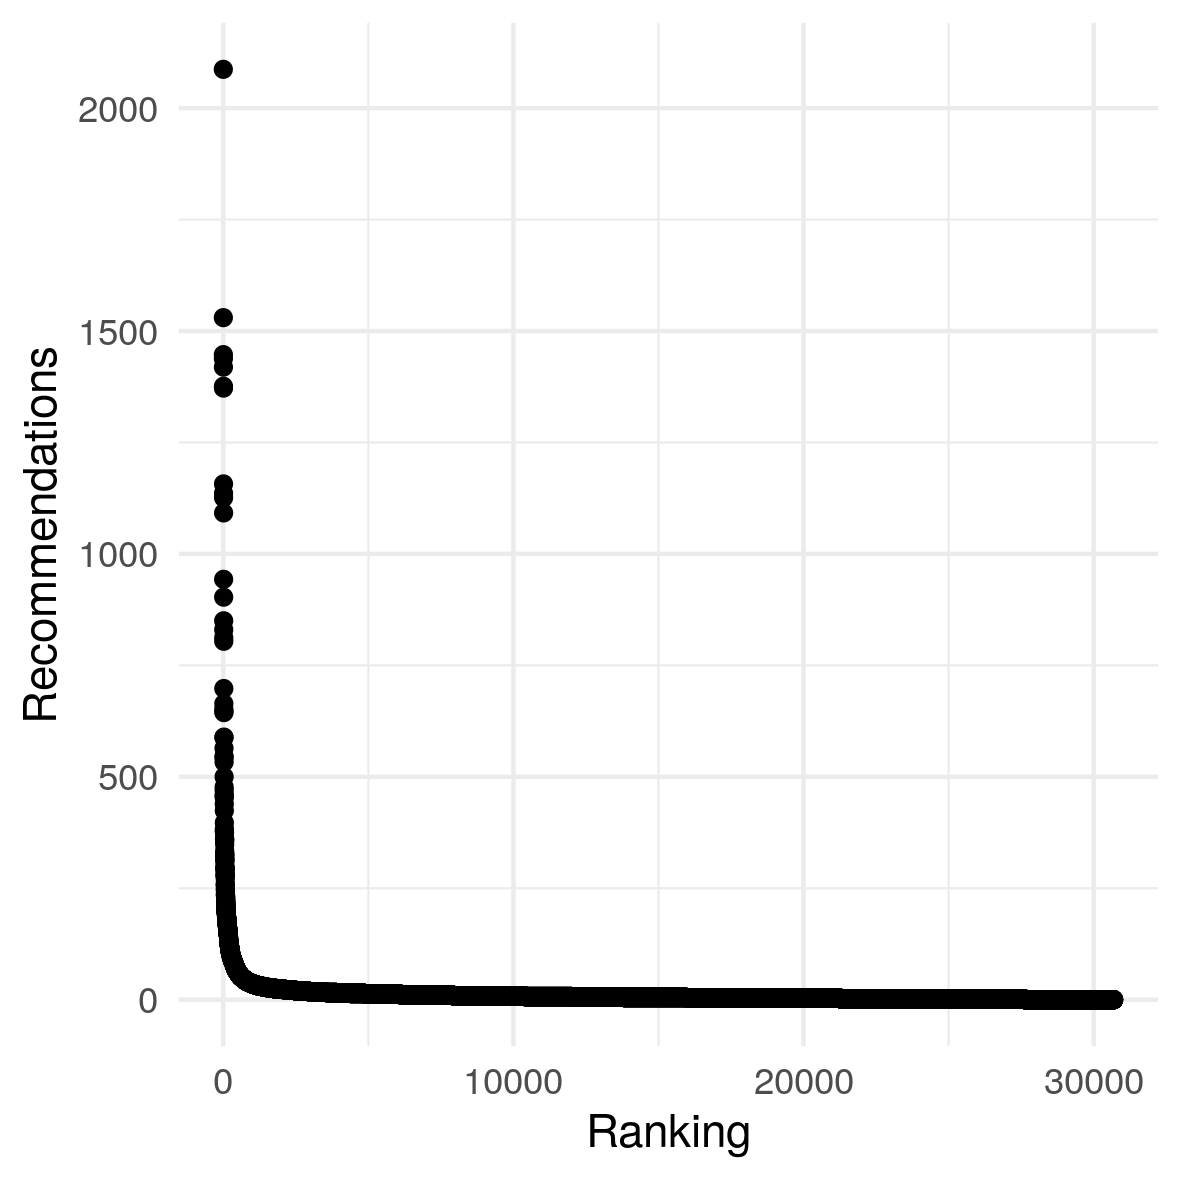
\includegraphics[width=\textwidth]{02_rec_vanilla}
    \caption{Rec. based on movie metadata.\label{fig:fig1:a}}
  \end{subfigure}
  \begin{subfigure}{0.45\textwidth}
    \centering
    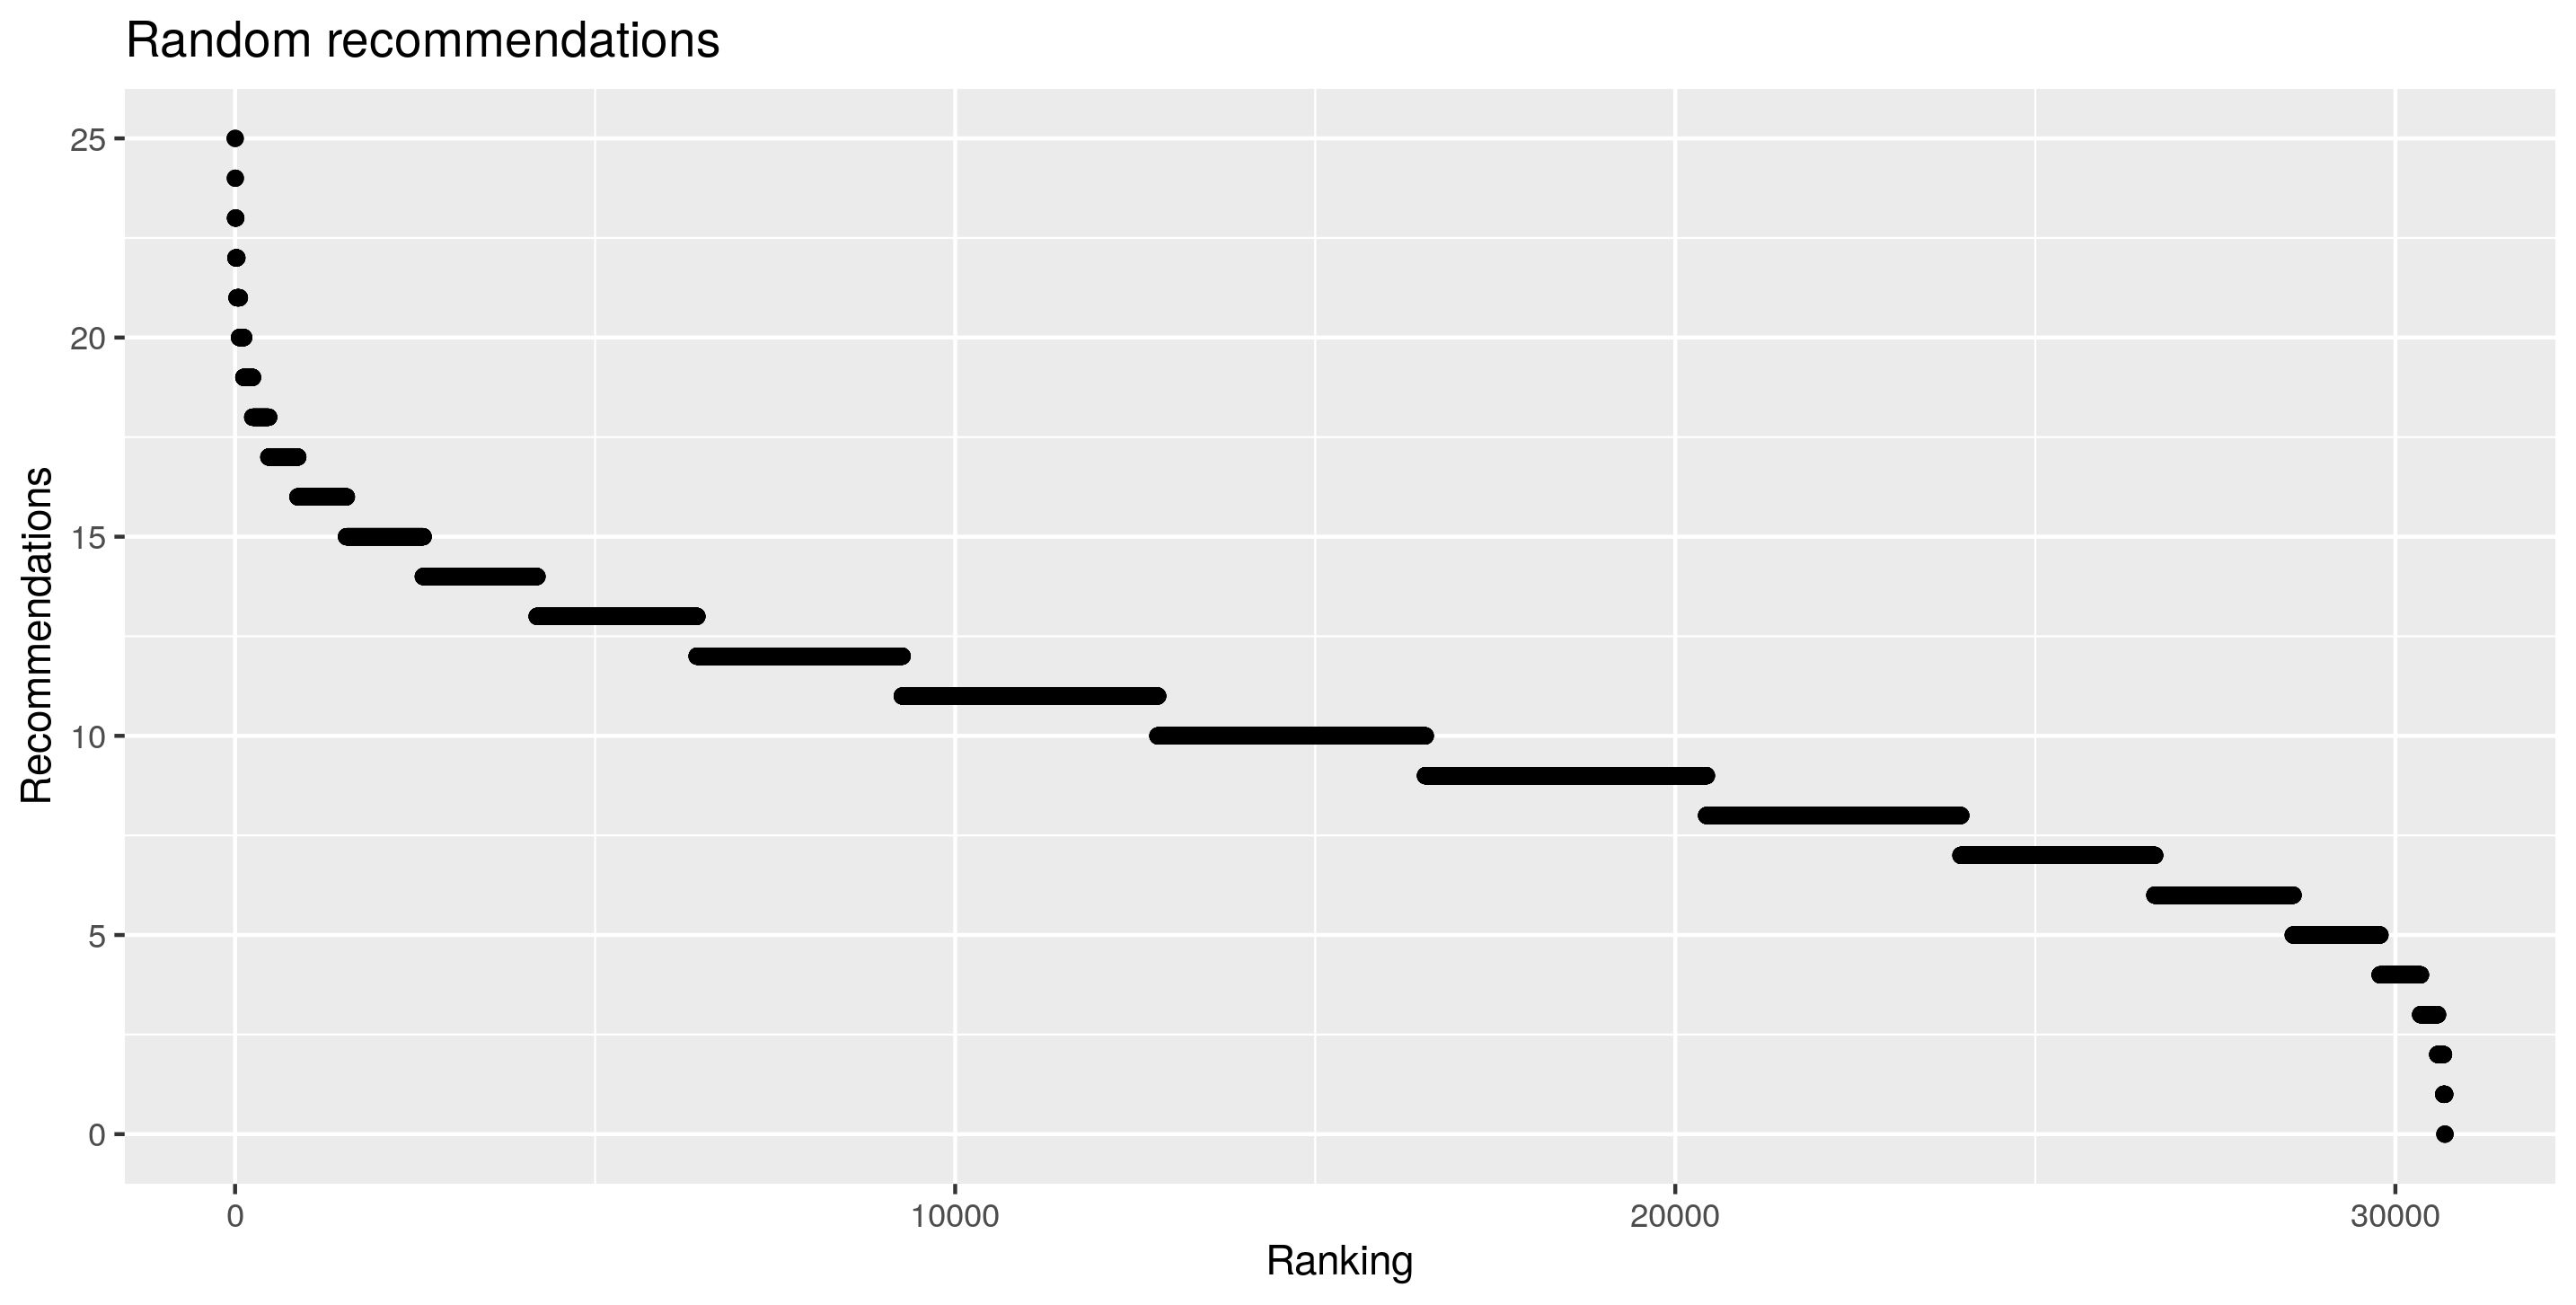
\includegraphics[width=\textwidth]{16_rec_random}
    \caption{Random recommendations.\label{fig:fig1:b}}
  \end{subfigure}
  \caption{Vanilla recommendation model and control.\label{fig:fig1}}
\end{figure}

For comparison, Figure~\ref{fig:fig1:b} is the same visualization for the
trivial model (sampling $k$ movies at random when asked for a recommendation).
The number of times each movie appeared in the final list of all recommendations
averaged, evidently, $k$, with an appearance very similar to that of the CDF of
the normal distribution. The ``most recommended'' movie appeared 25 times in the
final list, while the ``least recommended'' movie did not appear at all.
However, the distribution of the vanilla model differs immensely: the movie
ranked number 1 appeared more than 2000 times in the final list, with an almost
exponential decrease in the number of appearances from then on.

In order to better understand this phenomenon, more models were trained and
analyzed. Since all visualizations present exactly the same quantities, obtained
in the exact same way, all of them can be compared.

\begin{figure}
  \centering
  \begin{subfigure}{0.3\textwidth}
    \centering
    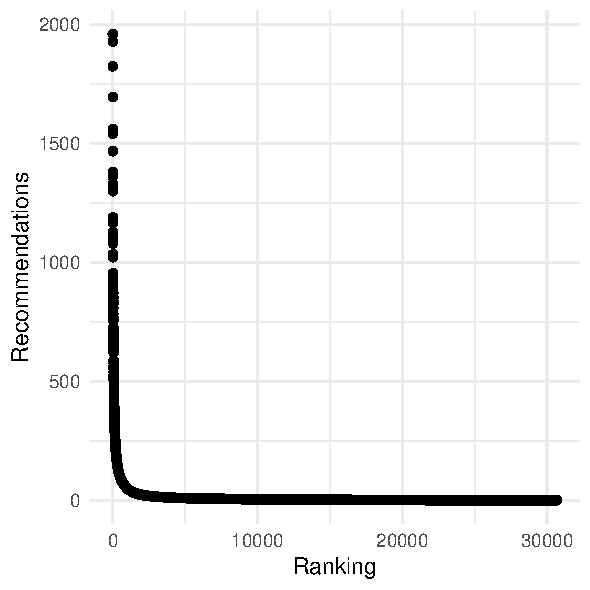
\includegraphics[width=\textwidth]{03_rec_cutoff_med}
    \caption{Cutoff $n \leqslant 5$.\label{fig:fig2:a}}
  \end{subfigure}
  \begin{subfigure}{0.3\textwidth}
    \centering
    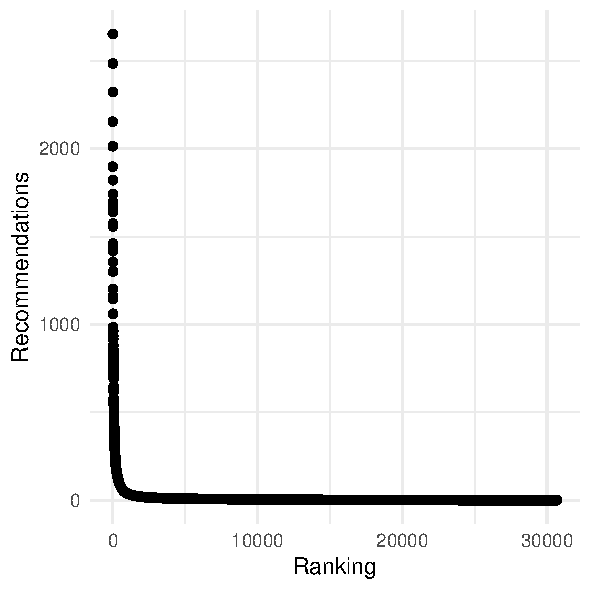
\includegraphics[width=\textwidth]{04_rec_cutoff_low}
    \caption{Cutoff $n \leqslant 2$.\label{fig:fig2:b}}
  \end{subfigure}
  \begin{subfigure}{0.3\textwidth}
    \centering
    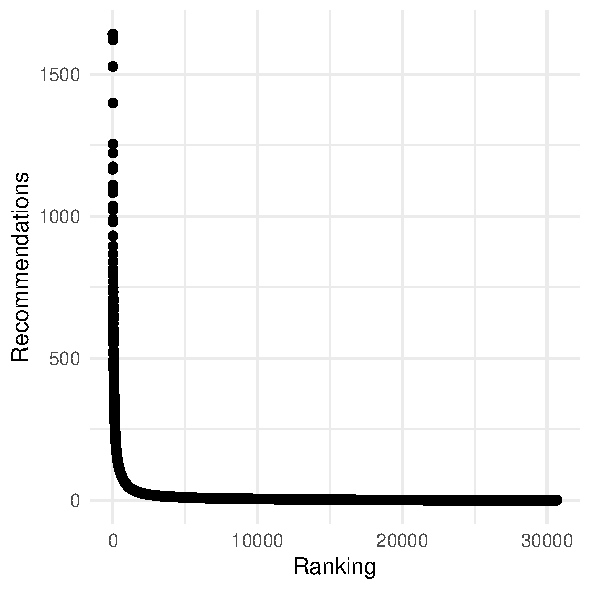
\includegraphics[width=\textwidth]{05_rec_cutoff_high}
    \caption{Cutoff $n \leqslant 8$.\label{fig:fig2:c}}
  \end{subfigure}
  \caption{Vanilla model with cutoff point.\label{fig:fig2}}
\end{figure}

\begin{figure}
  \centering
  \begin{subfigure}{0.3\textwidth}
    \centering
    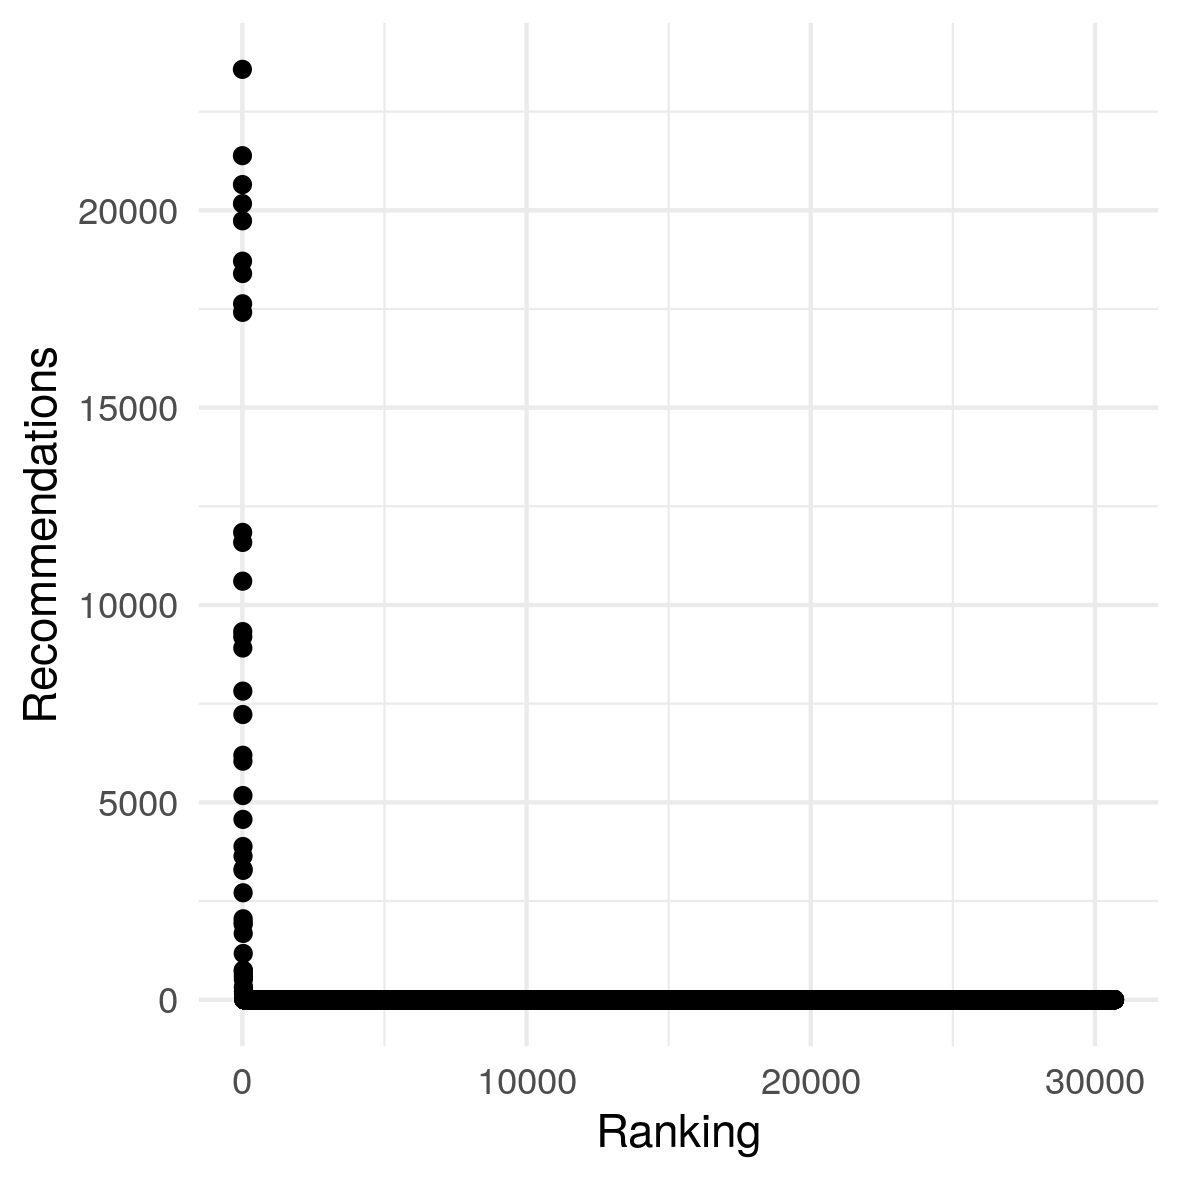
\includegraphics[width=\textwidth]{06_rec_cosine}
    \caption{Cosine distance.\label{fig:fig3:a}}
  \end{subfigure}
  \begin{subfigure}{0.3\textwidth}
    \centering
    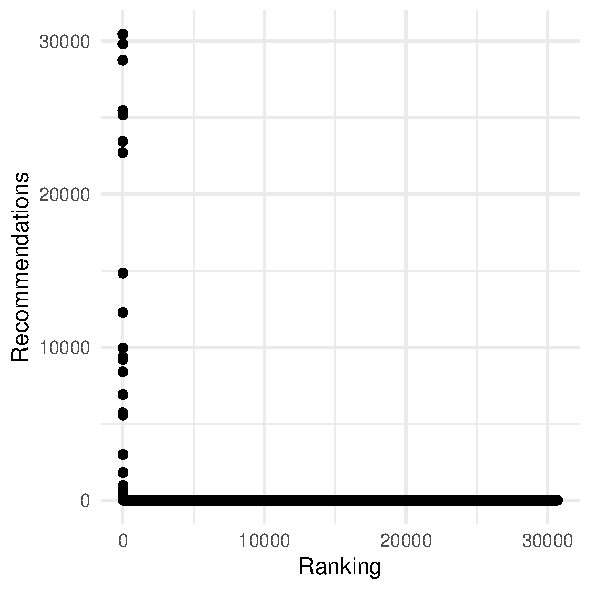
\includegraphics[width=\textwidth]{07_rec_euclidean}
    \caption{Euclidean distance.\label{fig:fig3:b}}
  \end{subfigure}
  \begin{subfigure}{0.3\textwidth}
    \centering
    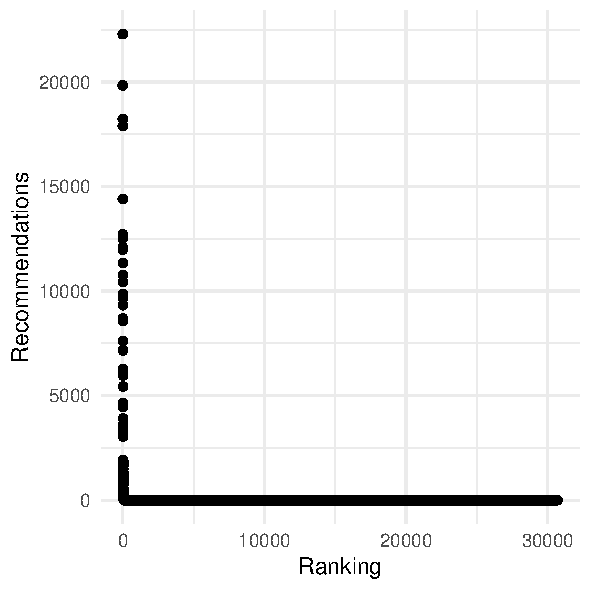
\includegraphics[width=\textwidth]{08_rec_manhattan}
    \caption{Manhattan distance.\label{fig:fig3:c}}
  \end{subfigure}
  \caption{Using distances instead of cosine similarity.\label{fig:fig3}}
\end{figure}

\begin{figure}
  \centering
  \begin{subfigure}{0.3\textwidth}
    \centering
    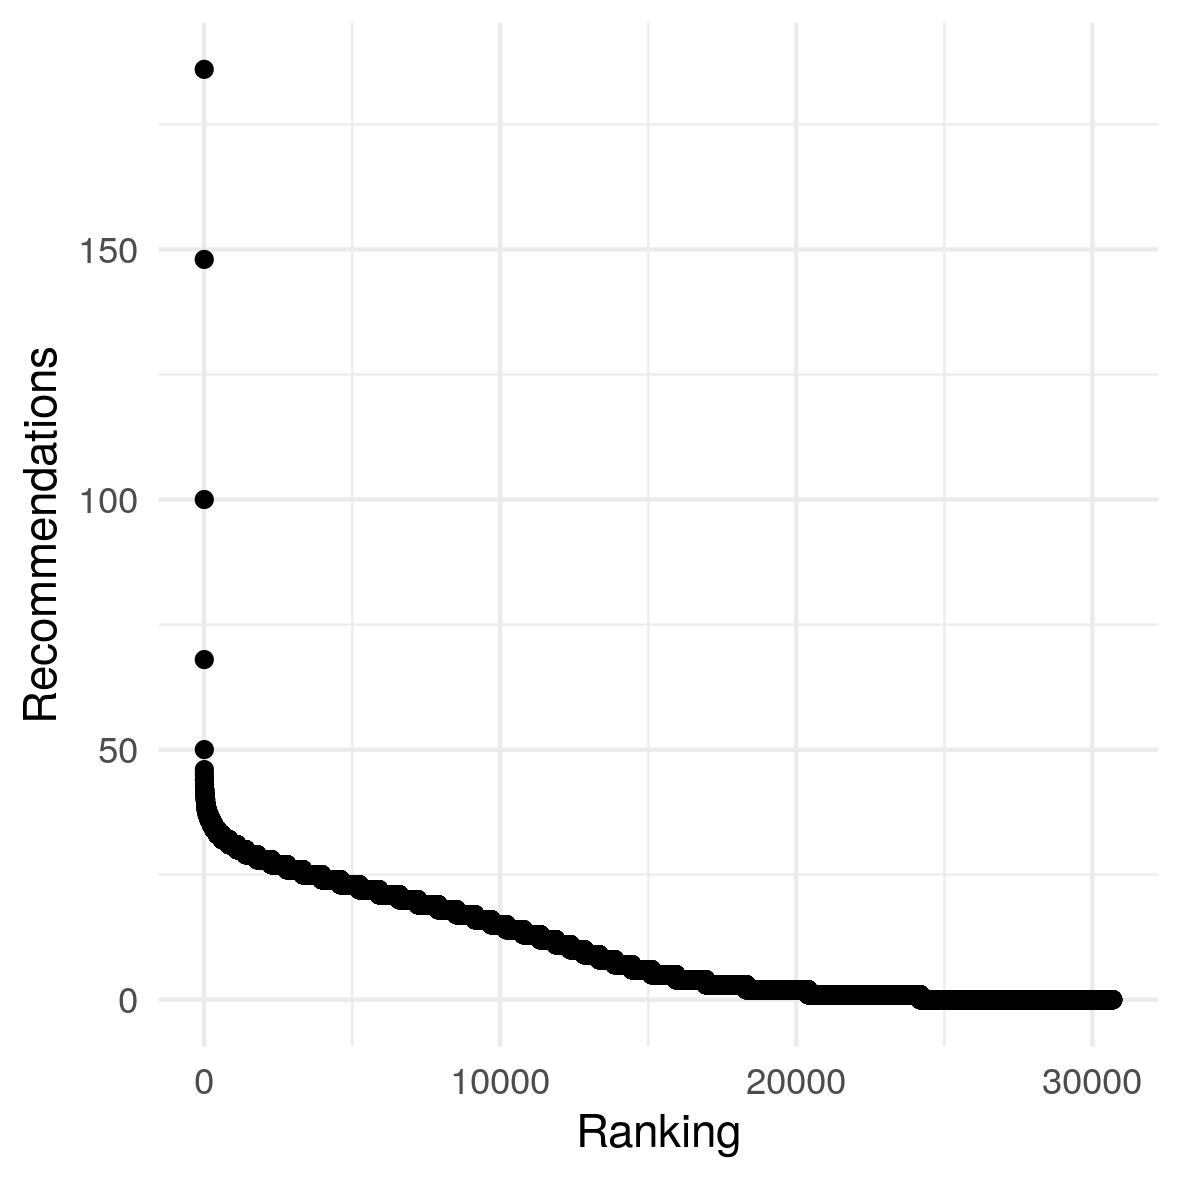
\includegraphics[width=\textwidth]{11_rec_p}
    \caption{$P(w) = P(V_w)$.\label{fig:fig4:a}}
  \end{subfigure}
  \begin{subfigure}{0.3\textwidth}
    \centering
    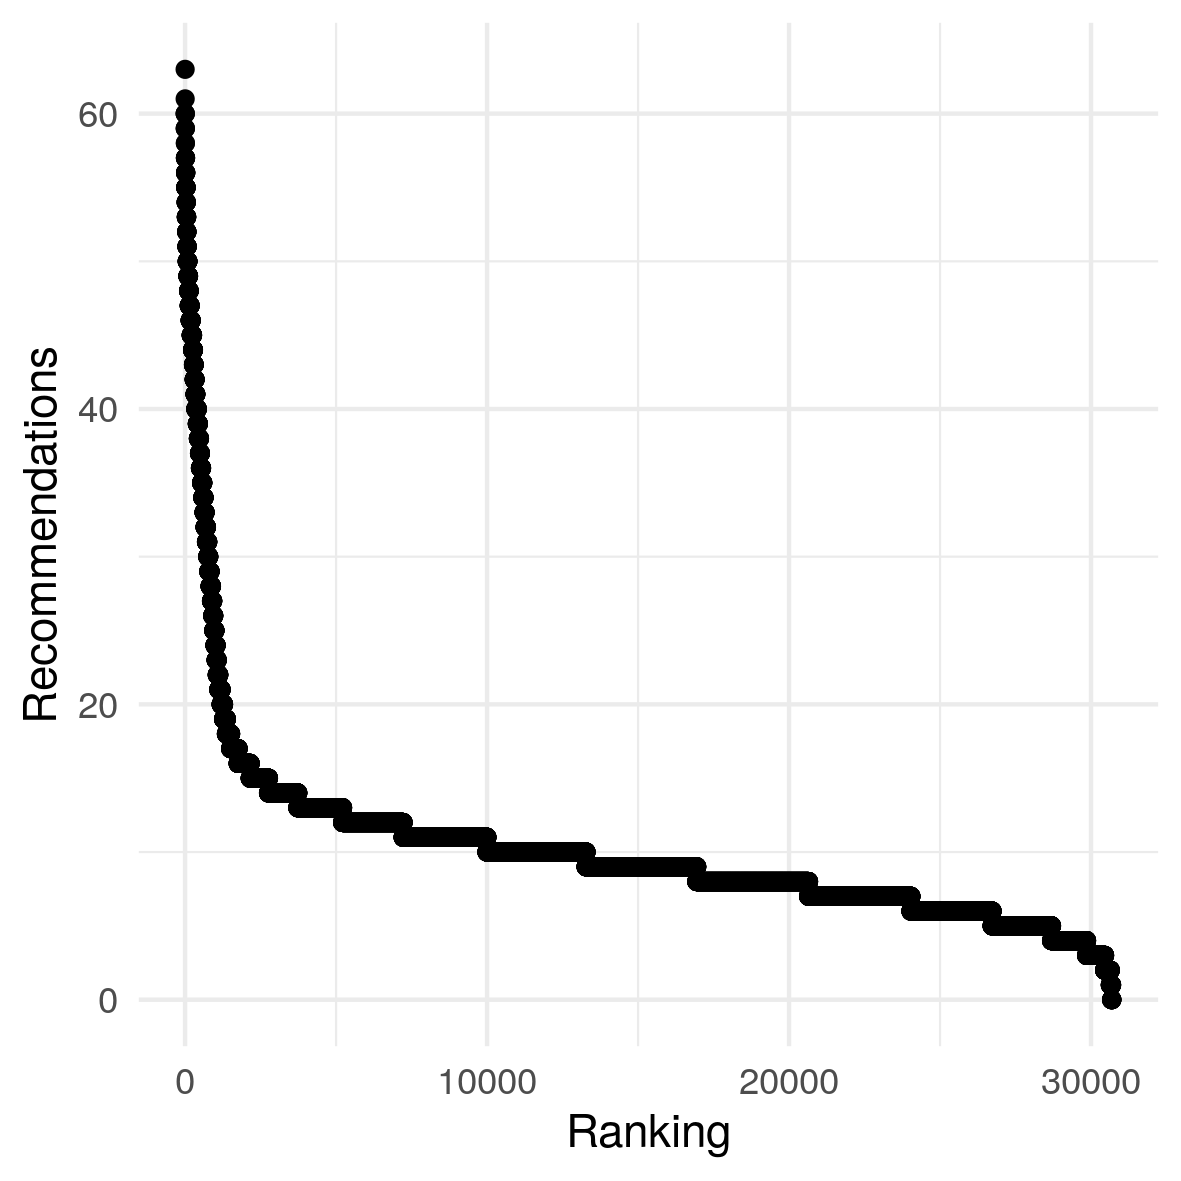
\includegraphics[width=\textwidth]{12_rec_p10}
    \caption{$P(w) = 10 \times P(V_w)$.\label{fig:fig4:b}}
  \end{subfigure}
  \begin{subfigure}{0.3\textwidth}
    \centering
    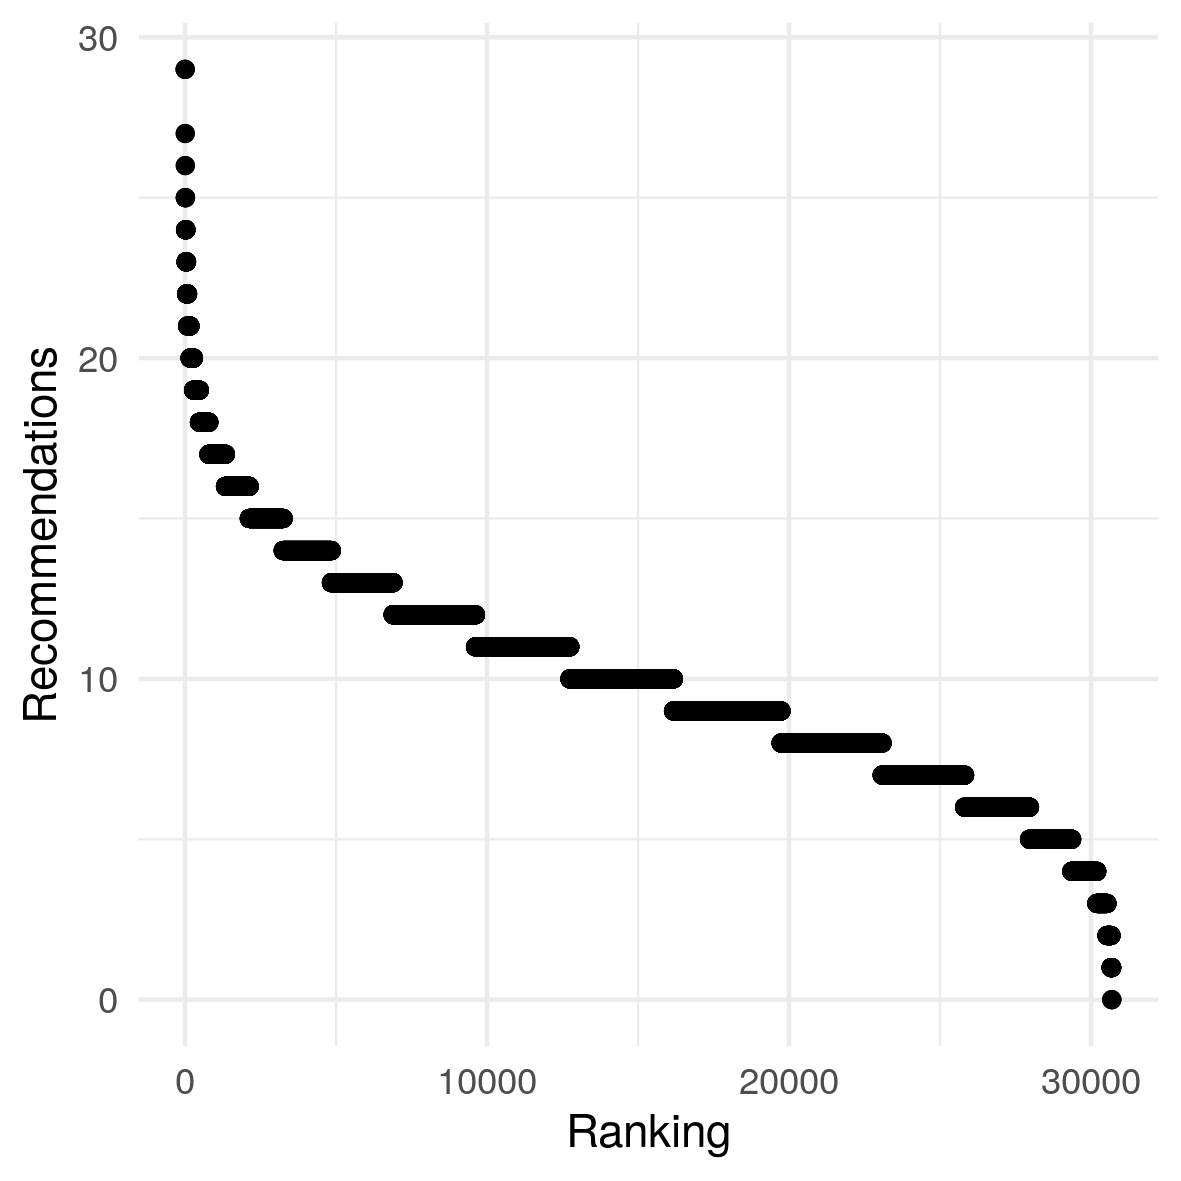
\includegraphics[width=\textwidth]{13_rec_p100}
    \caption{$P(w) = 100 \times P(V_w)$.\label{fig:fig4:c}}
  \end{subfigure}
  \caption{Random sample of words from metadata.\label{fig:fig4}}
\end{figure}

\begin{figure}
  \centering
  \begin{subfigure}{0.45\textwidth}
    \centering
    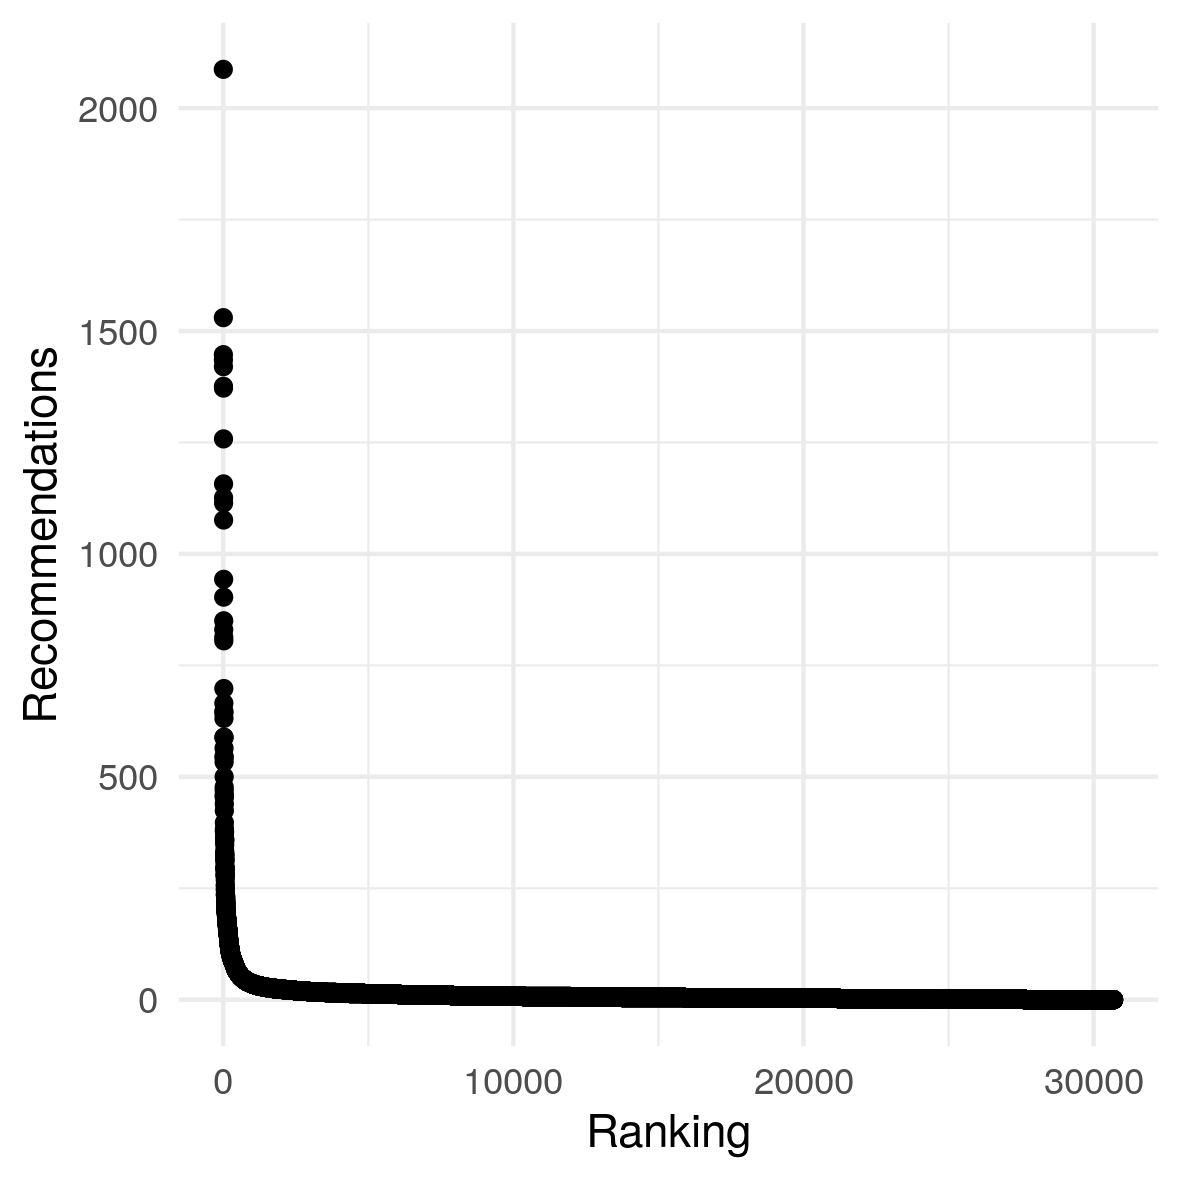
\includegraphics[width=\textwidth]{09_rec_artificial_movie}
    \caption{Artificial movie.\label{fig:fig5:a}}
  \end{subfigure}
  \begin{subfigure}{0.45\textwidth}
    \centering
    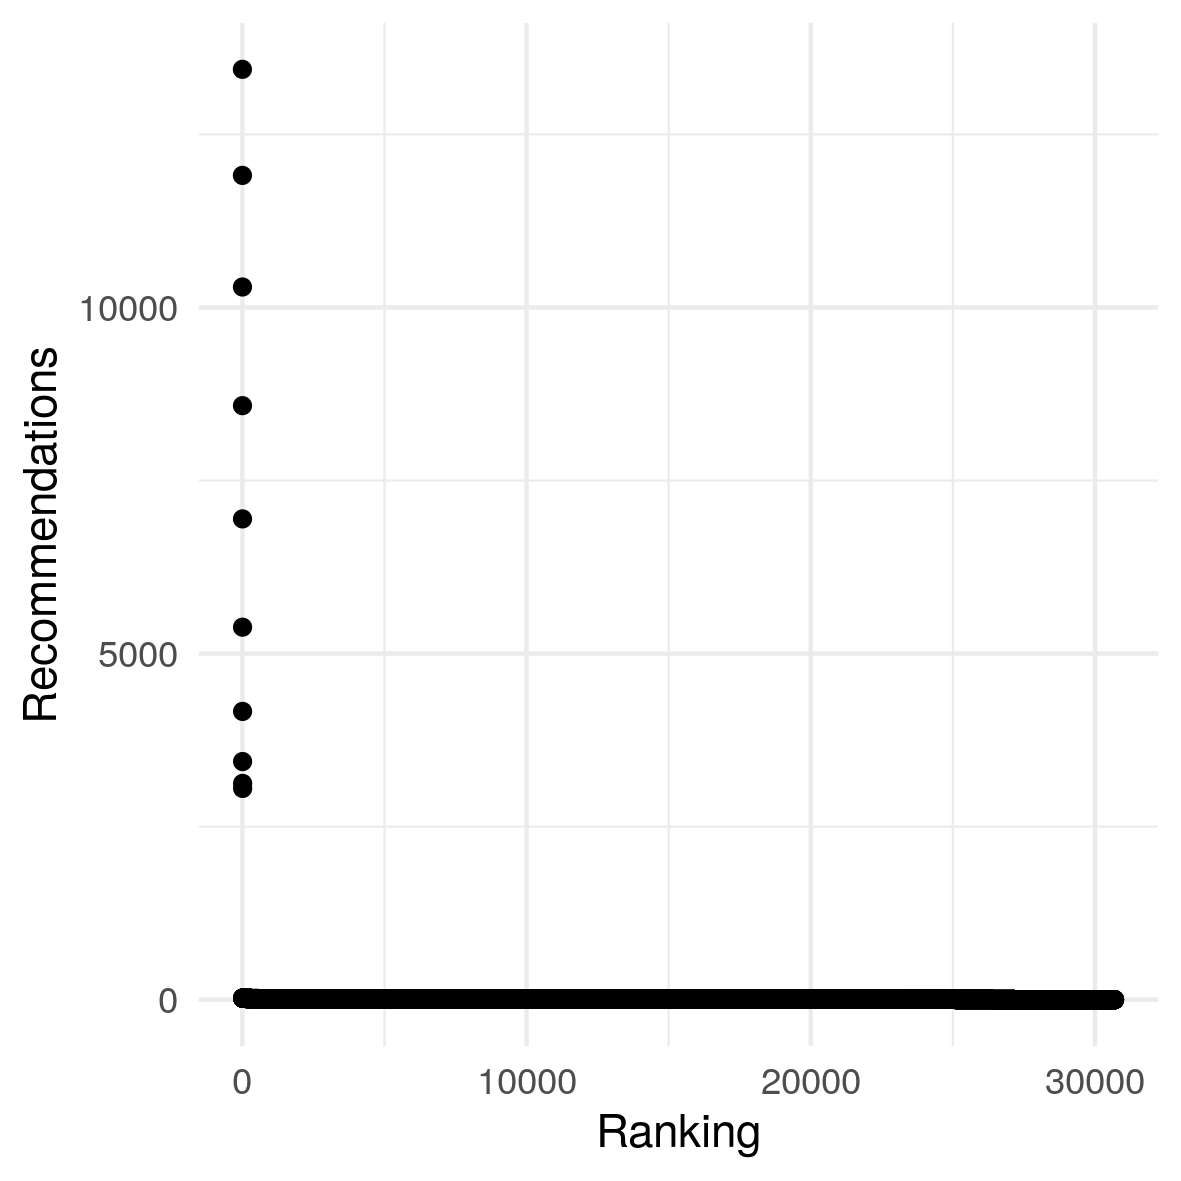
\includegraphics[width=\textwidth]{14_rec_long}
    \caption{Long and narrow.\label{fig:fig5:b}}
  \end{subfigure}
  \caption{Sanity checks.\label{fig:fig5}}
\end{figure}

\begin{figure}
  \centering
  \begin{subfigure}{0.45\textwidth}
    \centering
    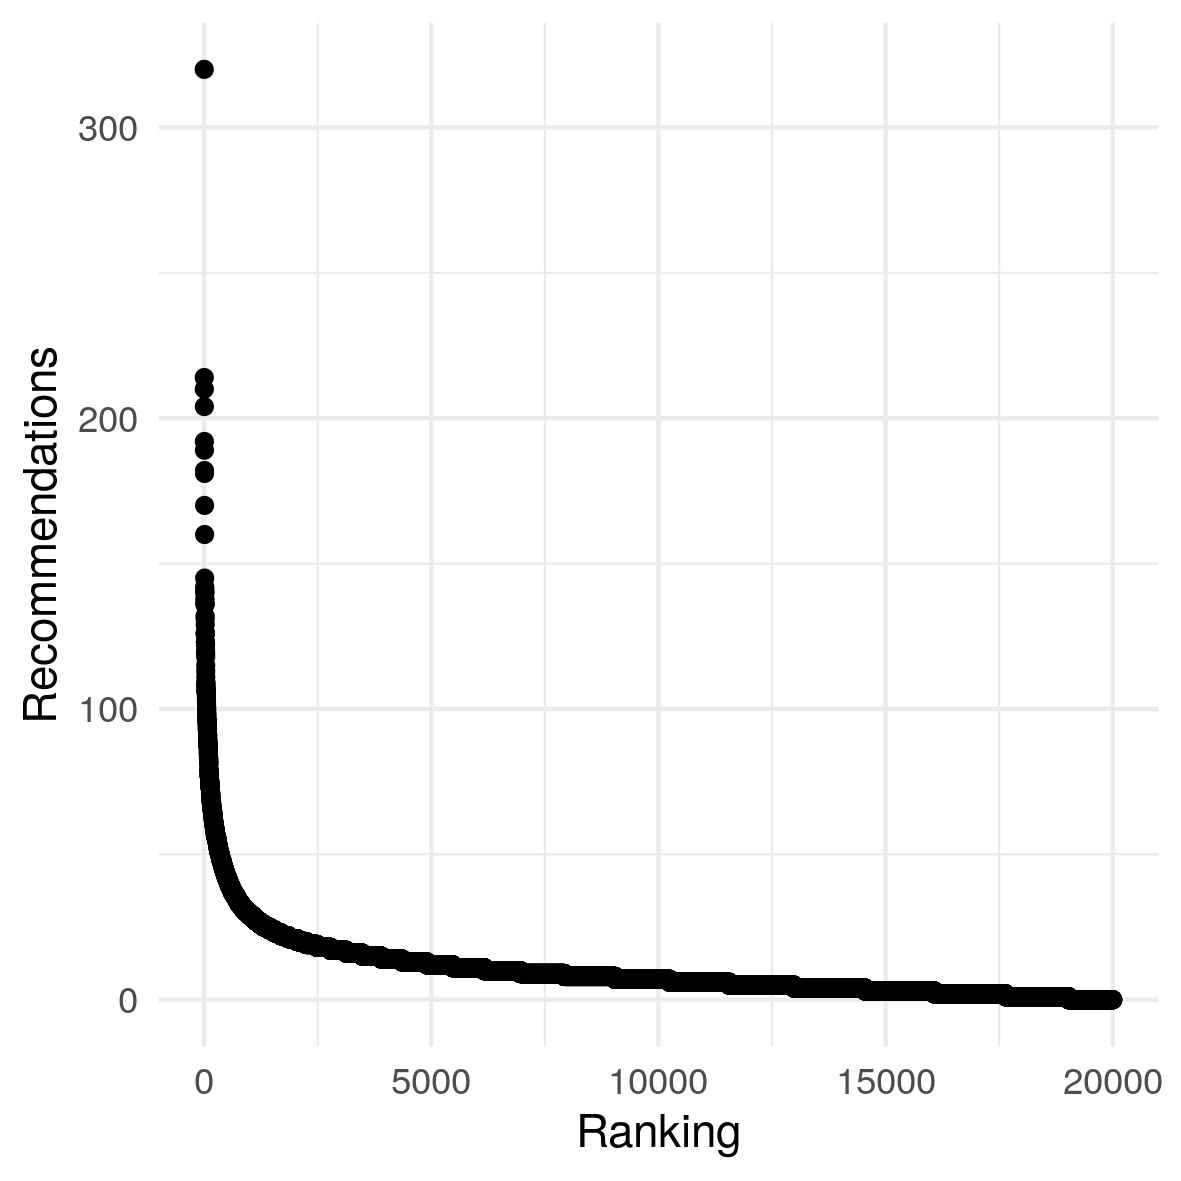
\includegraphics[width=\textwidth]{10_rec_books}
    \caption{Book dataset.\label{fig:fig6:a}}
  \end{subfigure}
  \begin{subfigure}{0.45\textwidth}
    \centering
    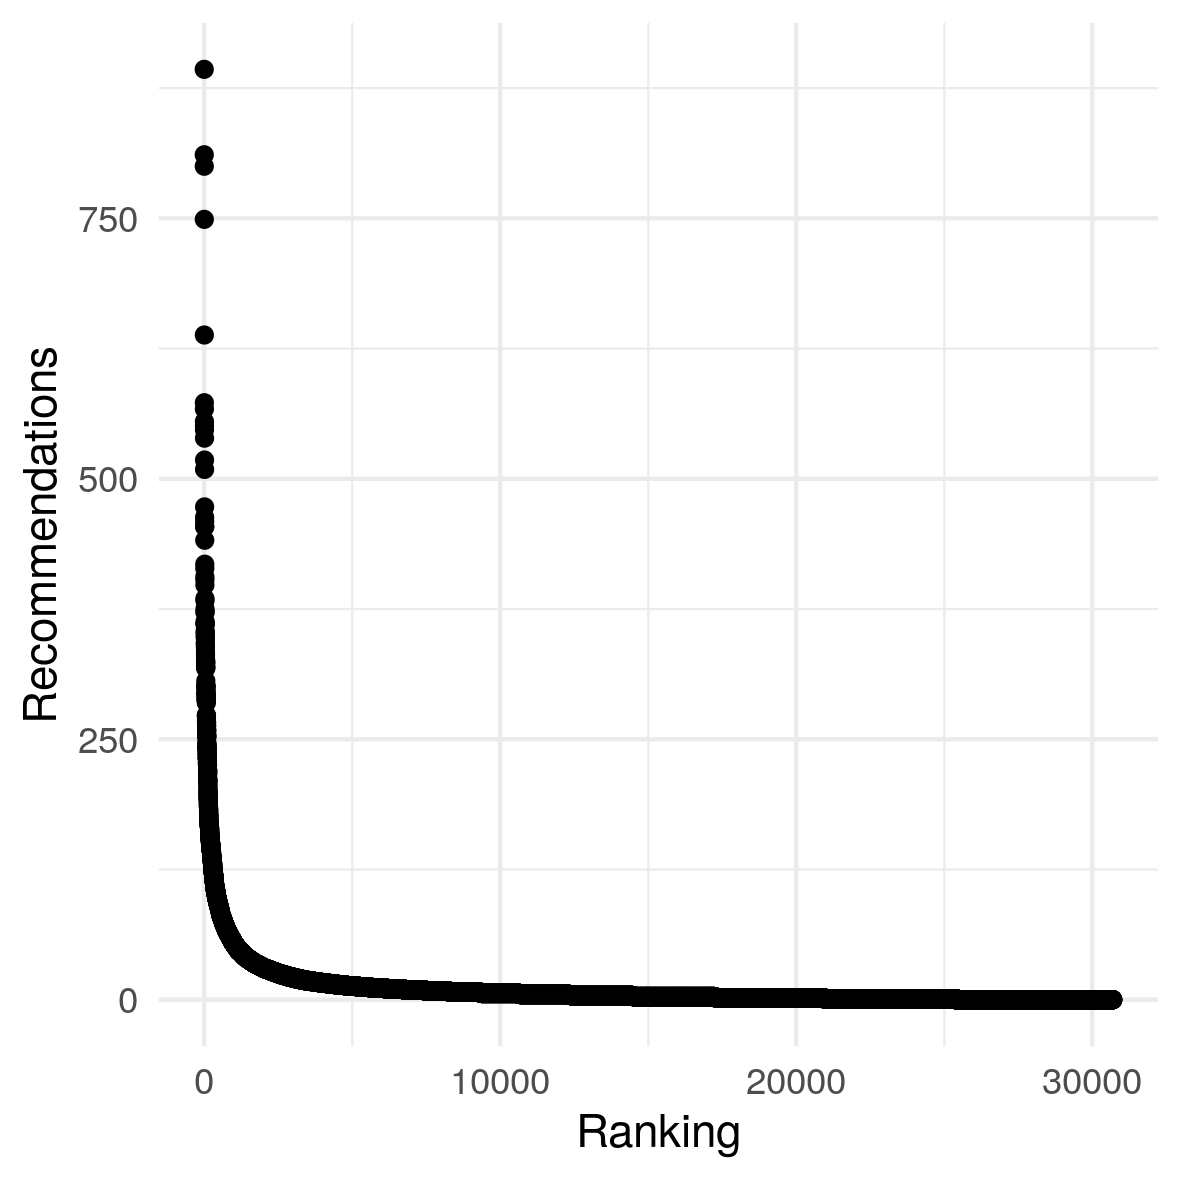
\includegraphics[width=\textwidth]{15_rec_mimic}
    \caption{Simulation of vanilla.\label{fig:fig6:b}}
  \end{subfigure}
  \caption{Confirmation of hypothesis.\label{fig:fig6}}
\end{figure}

\par
